% !TEX TS-program = xelatex

\documentclass[a4paper,12pt]{extarticle}
% !TEX TS-program = xelatex

% Document class and spacing
\renewcommand{\baselinestretch}{1.4}

% Packages
\usepackage{graphicx}
\usepackage{amsmath, amssymb}
\usepackage{geometry}
\usepackage{setspace}
\usepackage{fancyhdr}
\usepackage{titlesec}
\usepackage[colorlinks=true, linkcolor=darkblue, urlcolor=darkblue, citecolor=darkblue]{hyperref}
\usepackage[dvipsnames]{xcolor}
\usepackage{tcolorbox}
\usepackage{calc}
\usepackage{eso-pic}
\usepackage{fontspec}
\usepackage{natbib}
\usepackage{float}
\usepackage{caption}

\bibliographystyle{plain}

% English Fonts - Times New Roman
\setmainfont{Times New Roman}

% Colors
\definecolor{darkblue}{rgb}{.204,.353,.541}
\definecolor{lightblue}{RGB}{210, 227, 245}

% Section box command
\newcommand{\sectionbox}[1]{%
  \begin{tcolorbox}[colback=lightblue, colframe=lightblue, width=\linewidth, sharp corners]
    \color{darkblue} \eighteenpt \bfseries #1
  \end{tcolorbox}
}

% Section and subsection formatting
\titleformat{\section}
{\eighteenpt\bfseries}{} {0em} {\sectionbox}
\titlespacing{\section}{0pt}{12pt}{6pt}

\titleformat{\subsection}
{\color{darkblue}\sixteenpt\bfseries}
{\thesubsection}{1em}
{}

% Font size commands
\newcommand{\sixteenpt}{\fontsize{16pt}{18pt}\selectfont}
\newcommand{\eighteenpt}{\fontsize{18pt}{20pt}\selectfont}
\newcommand{\twentytwopt}{\fontsize{22pt}{24pt}\selectfont}
\newcommand{\twentyeightpt}{\fontsize{28pt}{30pt}\selectfont}

% Custom title page
\makeatletter
\def\maketitle{
  \begin{center}
    \begin{tabular}{ p{3cm} p{7cm} p{3.5cm} }
      
\includegraphics[width=3cm]{assets/images/logo.png} &
      \vspace{-3cm}
      \begin{center}
        {\sixteenpt{\textbf{University of Tehran}}\\[0.2cm]
          \sixteenpt{\textbf{College of Engineering}}\\[0.2cm]
        \sixteenpt{\textbf{Department of Electrical and Computer Engineering}}}
      \end{center}
      &
      
\includegraphics[width=3.5cm]{assets/images/eng-logo.png} 
    \end{tabular}

    \vspace{4cm}
    {\twentyeightpt \textbf{\CourseName}} \\
    \vspace{0.5cm}
    {\twentytwopt \textbf{\@title}} \\
    \vspace{2cm}
    {\eighteenpt \textbf{Instructors: Dr. Bahrak, Dr. Yaghoobzadeh}} \\
    \vspace{2cm}
    {\sixteenpt \textbf{Prepared by:}} \\
    \vspace{0.5cm}
    {\eighteenpt \textbf{\@author}} \\
    {\eighteenpt \textbf{Student No: \SNum}} \\
    \vfill
    {\sixteenpt \@date}
  \end{center}
}
\makeatother

\geometry{a4paper, margin=1in}
\graphicspath{{assets/images/}}

% --- Document Info ---
\newcommand{\CourseName}{Introduction to Data Science}
\newcommand{\assignNum}{1}
\title{Assignment \assignNum}

% Group Members Configuration
\author{
  Parsa Saeednia (810102460) \\
  Mohammad Hossein Mazaheri (810102585) \\
  Mohammad Reza Pirhadi (810102423)
}
\newcommand{\SNum}{Group Submission} % Overrides individual student number label
\date{\today}

\begin{document}
\pagenumbering{gobble}
\maketitle
\newpage
\tableofcontents
\newpage
\listoffigures
\newpage
\pagenumbering{arabic}

\section{Introduction}
This report outlines the findings and visualizations for Data Science Assignment 1. The project has three main parts: statistical sampling using 2D Gaussian distributions, creating interactive Tableau dashboards for Global Tuberculosis data, and improving a financial Power BI dashboard. The code for data processing and mathematical modeling is in the attached Jupyter Notebook.

\section{Task 1: Sampling and Inference}
This section visualizes the comparison between different sampling methods applied to a 2D Gaussian distribution.

\subsection{Direct Sampling Visualization}
% Insert your scatter plots or density plots from the Jupyter notebook here.
% \begin{figure}[H]
%     \centering
%     \includegraphics[width=0.7\textwidth]{direct_sampling.png}
%     \caption{Direct Sampling of the 2D Gaussian Distribution}
%     \label{fig:direct_sample}
% \end{figure}

\subsection{Langevin Dynamics Sampling}
% \begin{figure}[H]
%     \centering
%     \includegraphics[width=0.7\textwidth]{langevin_dynamics.png}
%     \caption{Sampling generated via Langevin Dynamics}
%     \label{fig:langevin_sample}
% \end{figure}

\subsection{Comparative Analysis}
% Discuss the differences in the visual spread, convergence, or accuracy between the two methods here.

\section{Task 2: Tableau Dashboard Storytelling}
This section explains how we prepared our data, built the interactive dashboards, and created a clear story to analyze the Global Tuberculosis (TB) data.

\subsection{Data Integration \& Preparation}
To add region and location details to our main disease data, we combined three files in Tableau:
\begin{itemize}
    \item \texttt{TB\_Burden\_Country.csv}: Contains the main country-level TB data over time.
    \item \texttt{Region.csv}: Contains the official WHO regional groups.
    \item \texttt{Coordinate.csv}: Provides the Latitude and Longitude for mapping.
\end{itemize}

We used a \textbf{Left Outer Join} to connect the \texttt{Region} and \texttt{Coordinate} tables to the main \texttt{TB\_Burden} table. We linked them using the \textbf{"Country or territory name"} and \textbf{"ISO numeric code"}. We chose a Left Join to make sure we keep all the region and map data, even if some countries were missing TB data. This keeps our maps and regional groups working perfectly.

To keep our analysis accurate, we handled missing values (nulls) very carefully:
\begin{itemize}
    \item \textbf{Avoiding Fake Zeros}: We did not replace missing values with zeros (like using the \texttt{ZN} function). Changing missing data to absolute zeros creates wrong statistics. For example, if we put zero for missing HIV data, it would incorrectly lower the averages and give us wrong results. 
    \item \textbf{Filtering Out Nulls}: Instead, we removed null records using a \texttt{Non-null values} filter. This makes sure our charts, averages, and trend lines only show real, reported data. For the heatmap, we simply showed "N/A" to show that data was not reported.
\end{itemize}

\subsection{Dashboard Interactions}
To make the dashboards easy to explore and analyze, we added several interactive filtering actions across the charts:

\begin{itemize}
    \item \textbf{Dashboard 1 (The Global Footprint)}: We used a two-way filter between the Regional Treemap and the World Map. Selecting a region on the Treemap filters the map to show only those countries. Conversely, clicking a country on the map highlights its region in the Treemap. We also included a \textbf{Year Slider} so users can move back and forth through time to watch how the disease spreads globally.
    
    \item \textbf{Dashboard 2 (The Syndemic)}: Selecting a specific region's bar in the ``Co-Infection Burden'' chart automatically filters the ``Mortality Accelerator'' scatter plot. This allows the user to temporarily hide other regions and focus strictly on the relationship between HIV and TB for the selected area.
    
    \item \textbf{Dashboard 3 (System Efficacy)}: We linked three charts together using filter actions. Clicking a square in the ``Diagnostic Blindspots'' heatmap isolates that country as a single dot on the ``Detection vs. Survival'' scatter plot, and vice versa. Furthermore, clicking any country in the ``Accountability List'' updates the other two charts to focus solely on it. To make the analysis easier and more actionable, we pre-filtered the Accountability List to only show the \textbf{Top 15 worst-performing countries}.
\end{itemize}

\subsection{Custom Calculated Fields}
To build the scatter plots, median lines, and dynamic colors, we created several custom calculated fields in Tableau. The core logic for these custom variables is structured as follows:

\begin{itemize}
    \item \texttt{Estimated incidence of TB (all forms)}: Represents the absolute estimated number of new and relapse Tuberculosis cases diagnosed within a given year.
    \begin{center}
    \begin{tcolorbox}[colback=white, colframe=lightblue, width=\linewidth, fontupper=\footnotesize\ttfamily, arc=3pt]
    ([Estimated total population number] \\
    \hspace*{1em} * [Estimated incidence (all forms) per 100 000 population]) \\
    / 100000
    \end{tcolorbox}
    \end{center}

    \item \texttt{Estimated mortality of TB (all forms) per 100k}: Specifies the standardized rate of TB-related deaths per 100,000 individuals in the population.
    \begin{center}
    \begin{tcolorbox}[colback=white, colframe=lightblue, width=\linewidth, fontupper=\footnotesize\ttfamily, arc=3pt]
    [Estimated mortality of TB cases (all forms, excluding HIV) \\
    \hspace*{1em} per 100 000 population] \\
    + [Estimated mortality of TB cases who are HIV-positive, \\
    \hspace*{1em} per 100 000 population]
    \end{tcolorbox}
    \end{center}

    \item \texttt{Total Deaths}: Calculates the total volume of mortality by converting the standardized absolute death counts.
    \begin{center}
    \begin{tcolorbox}[colback=white, colframe=lightblue, width=\linewidth, fontupper=\footnotesize\ttfamily, arc=3pt]
    [Estimated number of deaths from TB \\
    \hspace*{1em} (all forms, excluding HIV)] \\
    + [Estimated number of deaths from TB in people \\
    \hspace*{1em} who are HIV-positive]
    \end{tcolorbox}
    \end{center}

    \item \texttt{Global Median Detection}: Calculates the middle point for case detection to divide the scatter plot into distinct areas.
    \begin{center}
    \begin{tcolorbox}[colback=white, colframe=lightblue, width=\linewidth, fontupper=\footnotesize\ttfamily, arc=3pt]
    \{FIXED : MEDIAN( \\
    \hspace*{1em} IF NOT ISNULL([Case detection rate (all forms), percent]) \\
    \hspace*{1em} THEN [Case detection rate (all forms), percent] \\
    \hspace*{1em} END \\
    )\}
    \end{tcolorbox}
    \end{center}
    
    \item \texttt{Global Median Mortality}: Calculates the middle point for the mortality rate across all countries for a given year.
    \begin{center}
    \begin{tcolorbox}[colback=white, colframe=lightblue, width=\linewidth, fontupper=\footnotesize\ttfamily, arc=3pt]
    \{FIXED : MEDIAN( \\
    \hspace*{1em} IF NOT ISNULL([Estimated mortality of TB (all forms) \\
    \hspace*{2em} per 100 000 population]) \\
    \hspace*{1em} THEN [Estimated mortality of TB (all forms) \\
    \hspace*{2em} per 100 000 population] \\
    \hspace*{1em} END \\
    )\}
    \end{tcolorbox}
    \end{center}
    
    \item \texttt{Mortality Rate per 100k}: Standardizes the death count based on population size for fair comparisons.
    \begin{center}
    \begin{tcolorbox}[colback=white, colframe=lightblue, width=\linewidth, fontupper=\footnotesize\ttfamily, arc=3pt]
    [Estimated mortality of TB cases (all forms, excluding HIV) \\
    \hspace*{1em} per 100 000 population] \\
    + [Estimated mortality of TB cases who are HIV-positive, \\
    \hspace*{1em} per 100 000 population]
    \end{tcolorbox}
    \end{center}
    
    \item \texttt{Quadrant Color}: A conditional statement that assigns colors to countries based on where they fall compared to the global medians.
    \begin{center}
    \begin{tcolorbox}[colback=white, colframe=lightblue, width=\linewidth, fontupper=\footnotesize\ttfamily, arc=3pt]
    IF AVG([Case detection rate (all forms), percent]) \\
    \hspace*{1em} < ATTR([Global Median Detection]) \\
    AND AVG([Estimated mortality of TB (all forms) per 100 000 population]) \\
    \hspace*{1em} >= ATTR([Global Median Mortality]) \\
    THEN 'System Failure (Top Left)' \\[0.2cm]
    ELSEIF AVG([Case detection rate (all forms), percent]) \\
    \hspace*{1em} >= ATTR([Global Median Detection]) \\
    AND AVG([Estimated mortality of TB (all forms) per 100 000 population]) \\
    \hspace*{1em} >= ATTR([Global Median Mortality]) \\
    THEN 'Clinical Failure (Top Right)' \\[0.2cm]
    ELSEIF AVG([Case detection rate (all forms), percent]) \\
    \hspace*{1em} >= ATTR([Global Median Detection]) \\
    AND AVG([Estimated mortality of TB (all forms) per 100 000 population]) \\
    \hspace*{1em} < ATTR([Global Median Mortality]) \\
    THEN 'Success Zone (Bottom Right)' \\[0.2cm]
    ELSE 'Low Detection \& Low Mortality (Bottom Left)' \\
    END
    \end{tcolorbox}
    \end{center}
\ postseason
\end{itemize}

\subsection{The 6-Stage Story}
We built a 6-step Tableau Story to show our findings clearly, from a global view down to an action plan.

\begin{figure}[H]
    \centering
    
\includegraphics[width=0.95\linewidth]{stage1.png}
    \caption{Executive Summary and Data Lineage Overview.}
    \label{fig:stage1_executive}
\end{figure}

\begin{enumerate}
    \item \textbf{Stage 1: Executive Summary}
    \begin{itemize}
        \item \textit{Focus}: A clean page showing data sources and research architecture.
        \item \textit{Narrative}: This stage establishes the empirical foundation of the study using official, longitudinal datasets from the World Health Organization (WHO). It delineates the architectural lineage across all six major WHO epidemiological regions (AFR, AMR, EMR, EUR, SEA, WPR). By clearly mapping out the core metrics—such as incidence, prevalence, all-form mortality, and HIV co-infection—before diving into the analytics, this stage establishes data transparency, ensures scientific credibility, and sets a structured framework for the entire analytical narrative.
    \end{itemize}
\end{enumerate}

\begin{figure}[H]
    \centering
    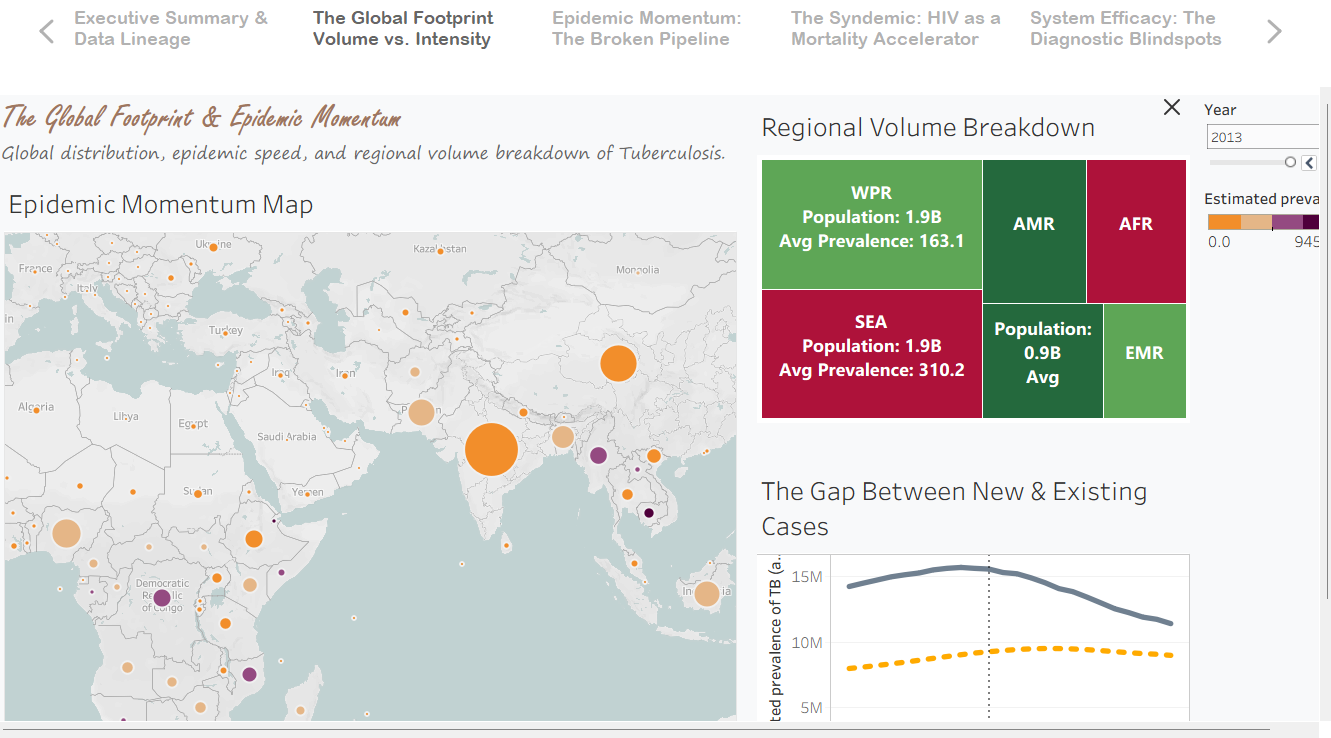
\includegraphics[width=0.95\linewidth]{stage2.png}
    \caption{The Global Footprint Dashboard: Volume vs. Intensity Analysis.}
    \label{fig:stage2_footprint}
\end{figure}

\begin{enumerate}
    \setcounter{enumi}{1}
    \item \textbf{Stage 2: The Global Footprint}
    \begin{itemize}
        \item \textit{Focus}: Bubble Map and Regional Prevalence Treemap side-by-side.
        \item \textit{Narrative}: This stage unveils a critical epidemiological dichotomy between absolute case volume and infection intensity. High-population nations in the South-East Asia (SEA) and Western Pacific (WPR) regions, specifically giants like India and China, exhibit massive absolute case volumes represented by the large bubble sizes, driven by sheer population scale. Conversely, the African region (AFR) displays a disproportionately severe epidemiological intensity; despite lower absolute populations, its darker shading signifies extremely high per-capita prevalence rates. This highlights that while Asian nations require heavy infrastructural scaling, African nations demand urgent, targeted clinical interventions to lower infection density.
    \end{itemize}    
\end{enumerate}    

\begin{figure}[H]
    \centering
    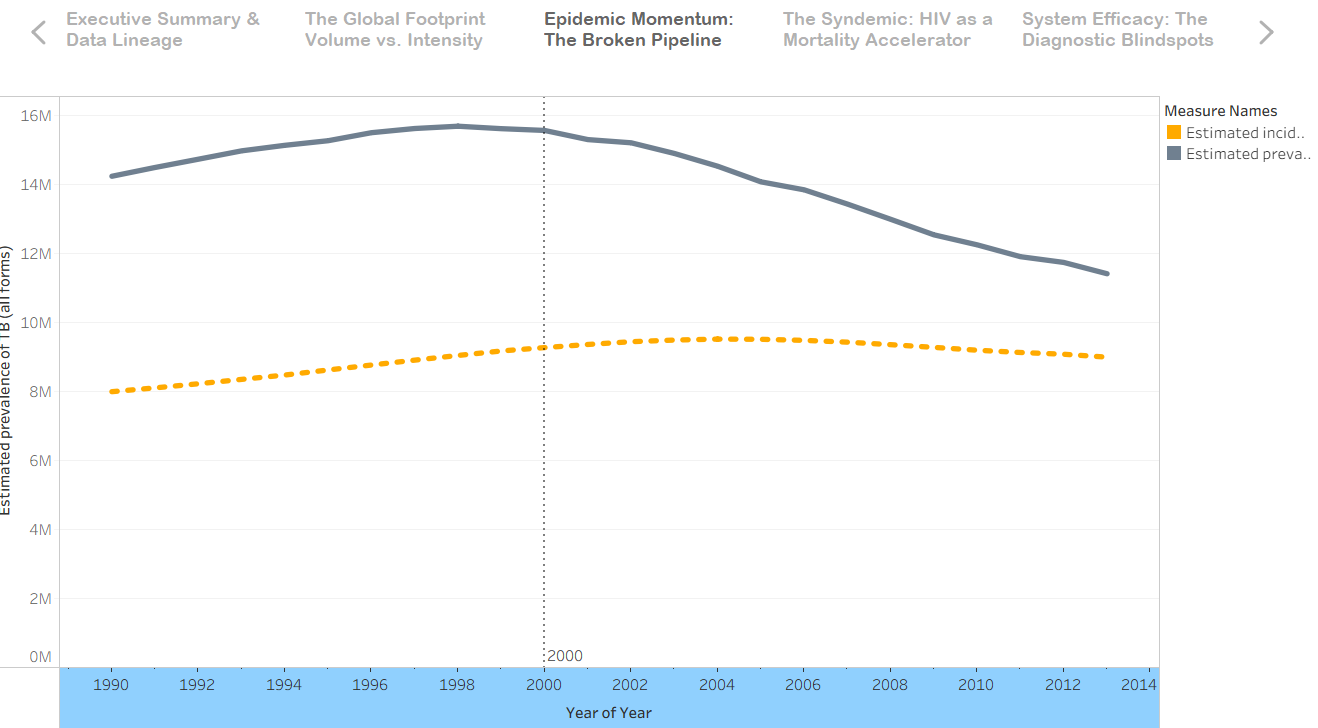
\includegraphics[width=0.95\linewidth]{stage3.png}
    \caption{Epidemic Momentum: The Broken Pipeline (Prevalence vs. Incidence Trends).}
    \label{fig:stage3_pipeline}
\end{figure}

\begin{enumerate}
    \setcounter{enumi}{2}
    \item \textbf{Stage 3: The Broken Pipeline}
    \begin{itemize}
        \item \textit{Focus}: Dual-Axis Line Chart tracking \texttt{Prevalence} vs. \texttt{Incidence} trends over time.
        \item \textit{Narrative}: This chart traces the historical trajectory of the epidemic, highlighting a vital paradigm shift marked by the vertical milestone line at the year 2000. Prior to this era, both prevalence and incidence were climbing rapidly. Post-2000, due to substantial advancements in medical technology, global sanitation, and targeted public health campaigns, the two curves begin to converge as total prevalence drops significantly. Concurrently, the slope of new infections (incidence) has flattened and started a gradual decline; however, it maintains a stubbornly persistent baseline because of explosive global population growth, signaling that although control mechanisms are working, transmission pipelines are not yet fully broken.
    \end{itemize}    
\end{enumerate}    

\begin{figure}[H]
    \centering
    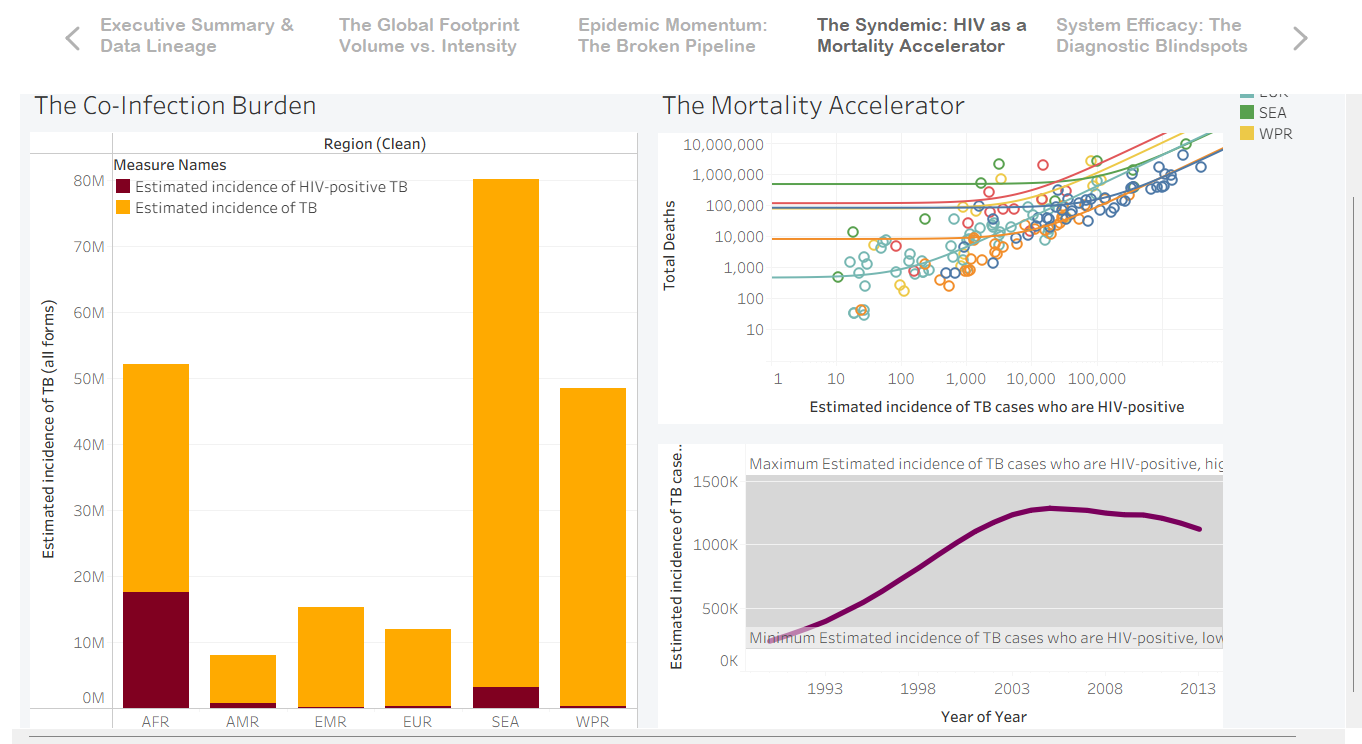
\includegraphics[width=0.95\linewidth]{stage4.png}
    \caption{The Syndemic: HIV Co-infection as a Mortality Accelerator.}
    \label{fig:stage4_syndemic}
\end{figure}

\begin{enumerate}
    \setcounter{enumi}{3}
    \item \textbf{Stage 4: HIV as an Accelerator}
    \begin{itemize}
        \item \textit{Focus}: Logarithmic Scatter Plot with regional trend lines coupled with a Co-Infection Burden Bar Chart.
        \item \textit{Narrative}: This stage investigates the deadly intersection of the TB-HIV syndemic, demonstrating how HIV acts as a catastrophic accelerator of human mortality. The log-scale scatter plot illustrates a tight, positive correlation between the incidence of HIV-positive TB cases and total deaths, proving that co-infection exponentially decreases patient survival rates. Regionally, the bar chart exposes the African region (AFR) as the epicenter of this dual crisis, holding an overwhelmingly large share of HIV-positive TB cases compared to other regions like South-East Asia (SEA). This demands an integrated clinical approach where HIV antiretroviral therapies and TB antibiotics are co-administered simultaneously.
    \end{itemize}    
\end{enumerate}

\begin{figure}[H]
    \centering
    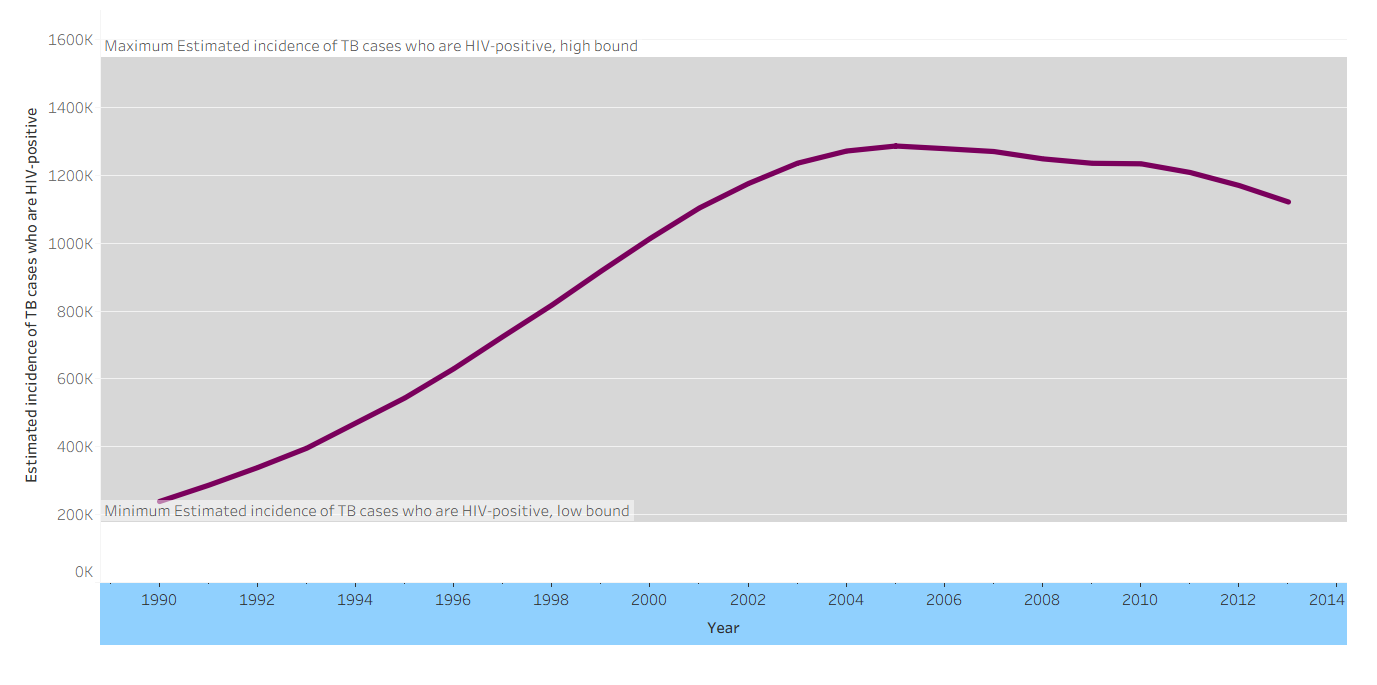
\includegraphics[width=0.95\linewidth]{stage5.png}
    \caption{Epidemiological Variance: Longitudinal Decline of the Estimation Confidence Band.}
    \label{fig:stage5_confidence_band}
\end{figure}


\begin{enumerate}
    \setcounter{enumi}{4}
    \item \textbf{Stage 5: Estimation Confidence Band}
    \begin{itemize}
        \item \textit{Focus}: Empirical Uncertainty Bounds and Epidemiological Variance.
        \item \textit{Narrative}: This visualization tracks the statistical confidence intervals of global TB estimates, exposing a profound structural turning point around the year 2006. Prior to this era, the wider confidence bands reflected substantial data volatility and lower tracking precision across developing healthcare infrastructures. Post-2006, the prominent downward trajectory of the estimation band signifies a major expansion in data precision. This drop is driven by two catalyst factors: the digitization of global surveillance systems which standardized country-level reporting, and the emergence of revolutionary molecular diagnostic technologies. By replacing mathematical projections with empirical, active case tracking, the statistical margin of error collapsed, reinforcing the scientific reliability of global intervention frameworks.
    \end{itemize}
\end{enumerate}

\begin{figure}[H]
    \centering
    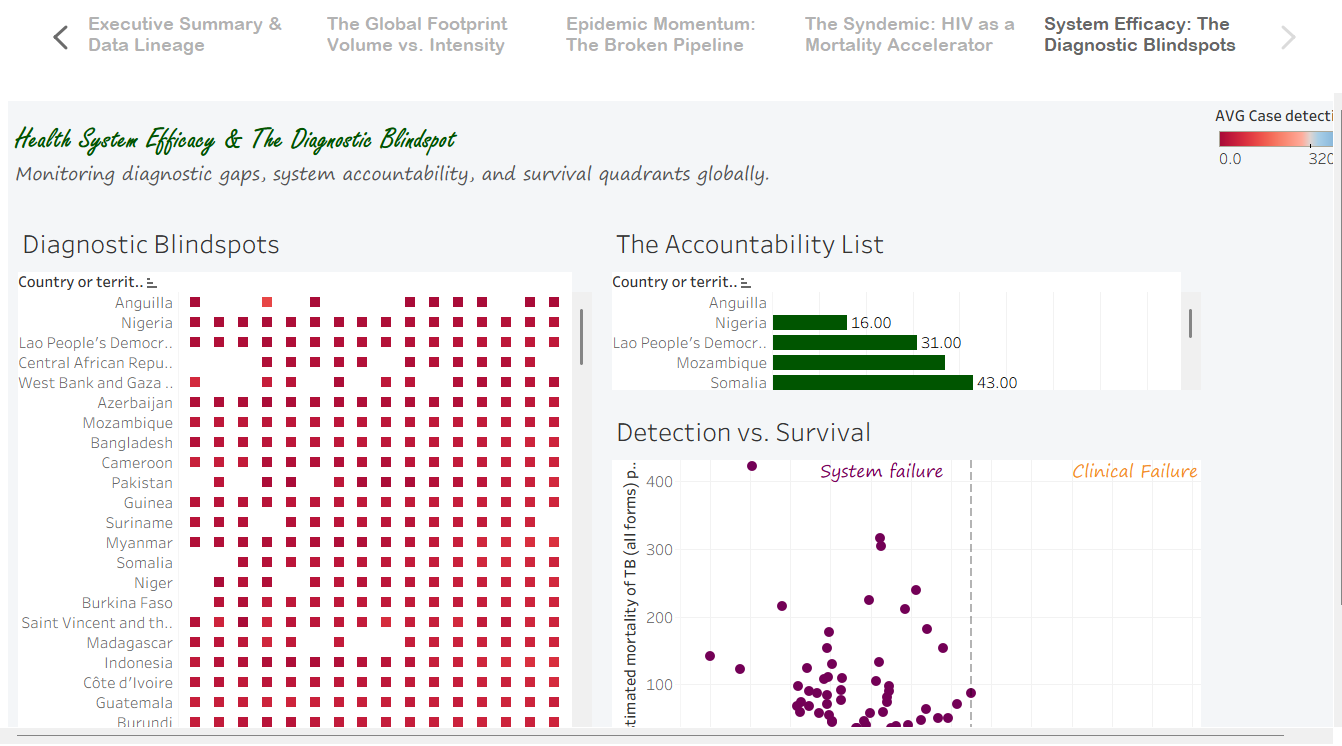
\includegraphics[width=0.95\linewidth]{stage6.png}
    \caption{System Efficacy: Heatmap of Global Diagnostic Blindspots.}
    \label{fig:stage6_blindspots}
\end{figure}

\begin{enumerate}
    \setcounter{enumi}{5}
    \item \textbf{Stage 6: Finding the Blindspots}
    \begin{itemize}
        \item \textit{Focus}: Longitudinal Heatmap of case detection rates.
        \item \textit{Narrative}: This stage shifts focus from clinical severity to healthcare delivery infrastructure by mapping structural failures via a diagnostic heatmap. The persistent red indicators over consecutive years flag critical "blindspots" where case detection rates routinely plummet below acceptable thresholds in countries like Nigeria, Mozambique, and Somalia. This visualization proves that the primary bottleneck in these healthcare systems is a systematic failure to screen, diagnose, and register active cases within communities, rather than a mere shortage of pharmaceutical treatments. Without active case-finding and diagnostic expansion, hidden reservoirs of the disease will continue to drive community transmission.
    \end{itemize}    
\end{enumerate}    

\begin{figure}[H]
    \centering
    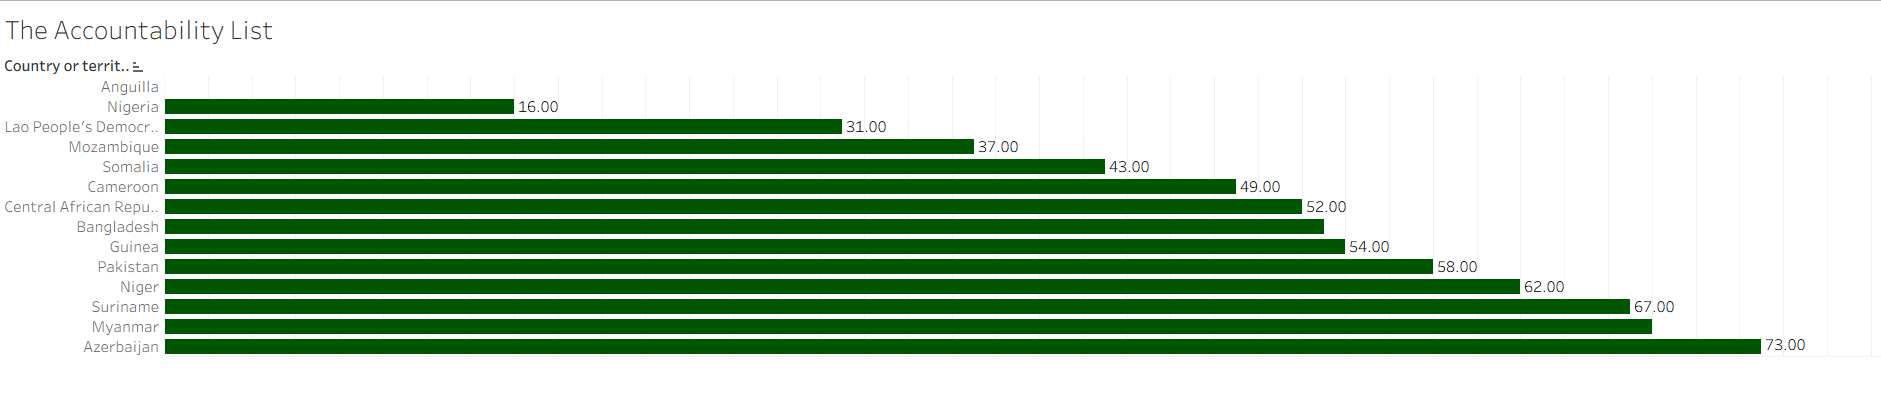
\includegraphics[width=0.95\linewidth]{stage7.png}
    \caption{Action Plan: Detection vs. Survival Quadrant Scatter Plot and Priority List.}
    \label{fig:stage7_action}
\end{figure}

\begin{enumerate}
    \setcounter{enumi}{6}
    \item \textbf{Stage 7: Action Plan}
    \begin{itemize}
        \item \textit{Focus}: Detection vs. Survival Quadrant Scatter Plot and a filtered Priority Accountability List.
        \item \textit{Narrative}: This final stage synthesizes previous insights into an actionable, data-driven governance framework by plotting nations along a "Detection vs. Survival" quadrant scatter plot. It isolates the most vulnerable countries within the critical "System Failure" quadrant—characterized by dangerously low case detection rates combined with high mortality. By coupling this with a prioritized "Accountability List" of the top 15 worst-performing nations (such as Nigeria and Somalia), the dashboard transcends descriptive analytics to provide a strategic blueprint for international aid. It recommends that global health funding must be reallocated away from generic programs and directed explicitly toward upgrading laboratory networks, molecular testing infrastructure, and community-based surveillance in these high-priority zones.
    \end{itemize}    
\end{enumerate}    

\subsection{Visual Design Principles}
To make the dashboard easy to read, we used standard design rules:
\begin{itemize}
    \item \textbf{Gestalt Principles (Grouping)}: We used a clean grid layout with white cards on a light gray background. This helps the user easily see which charts belong together. We also removed messy gridlines on line charts to make them easier to follow.
    \item \textbf{Colors and Sizes}: We used a calm color palette, keeping dark Purple only for danger zones so it catches the eye immediately. We also used bubble sizes to clearly show the number of cases. 
\end{itemize}

\section{Task 3: Power BI Dashboard Improvement}
This section details the enhancements made to the financial Power BI dashboard, focusing on advanced indicators and improved visual hierarchy.

\subsection{Original vs. Enhanced Dashboard}
% \begin{figure}[H]
%     \centering
%     \includegraphics[width=0.9\textwidth]{powerbi_enhanced.png}
%     \caption{Enhanced Financial Dashboard with improved KPIs and Layout}
%     \label{fig:powerbi_enhanced}
% \end{figure}

\subsection{Advanced Financial Indicators}
% Detail the new metrics you introduced and why they add business value.

\subsection{Design and UX Improvements}
% Explain what you changed visually to make the dashboard more readable.

\section{Task 4: Data Visualization Principles}

\subsection{Labeling: Clarity vs. Clutter}
In data visualization, labeling every data point can either be very helpful or create a lot of mess. We must use labels when exact numbers are important. For example, in our list of the 15 worst countries, seeing the exact percentage (like 42\%) is necessary for making decisions.

But, labels create too much visual clutter on a scatter plot with hundreds of dots. In these cases, overlapping text makes the chart unreadable. For busy charts, it is much better to hide the labels and use interactive tooltips when the user hovers over a point.

\subsection{Cognitive Load and Visual Simplicity}
To make the charts easier to read, we synchronized the dual-axis charts and hid the extra numbers. Usually, charts with two axes have different scales on the left and right, which makes them very confusing to read.

\begin{figure}[H]
    \centering
    \begin{tcolorbox}[colback=white, colframe=lightblue, arc=4pt, width=0.85\linewidth, left=15pt, right=15pt, top=10pt, bottom=10pt]
        \centering
        \textbf{Data-Ink Ratio Optimization Formula}
        \vskip 6pt
        $$\text{Data-Ink Ratio} = \frac{\text{Ink dedicated to critical data-information}}{\text{Total ink used to print the graphic}}$$
        \vskip 4pt
        \small By shortening long numbers (e.g., \textbf{1.4B} instead of \textbf{1,400,000,000}) and hiding the right-side axis header, we make the chart much cleaner.\end{tcolorbox}
    \caption{Tufte's Data-Ink Evaluation Protocol.}
    \label{fig:data_ink_box}
\end{figure}

By matching the left and right axes and hiding the right-side header, we remove useless text. This follows Edward Tufte’s \textbf{"Data-Ink Ratio"} rule, which says we should remove any ink that doesn't show new data. This also helps the eyes follow the lines smoothly without getting confused by two different number scales.

\end{document}